\subsection{重味夸克半轻子衰变}

在中等质量区间,来源于重味夸克半轻子衰变的双轻子对占了主要的部分。我们使用PYTHIA6作为模拟的产生子来得到模拟结果。由PYTHIA6产生的质子-质子对撞中的结果经过归一化和乘以$N_{bin}$后与介子模拟的结果加在一起后与最终的测量结果进行比较。在本小节中将对整个模拟过程进行详细介绍。因为在低能量下,相比于c夸克的截面b夸克的截面很小可以忽略不计,所以在本分析中仅对c夸克的贡献进行模拟。

对于PYTHIA6产生子,在本分析中基本沿用STAR的模拟设置,但对以下几个参数进行了调整:MSEL = 4(c trigger); PARP(91) = 1 $<k_T>$ = 1.0 GeV/c; PARP(61) = 1 (parton shower level tuning)
同时为了提高模拟的效率,对于产生的含c夸克的介子,在产生子当中将不含电子的衰变道关闭。

通过PYTHIA得到的来源于c夸克半轻子衰变的双电子分布经过式\ref{eq:Nor_c}归一化之后再与测量结果进行比较。其中$\sigma_{cc}$和$\sigma_{mb}$分别为金-金对撞中c夸克和最小无偏对撞的截面,$N_{bin}$为不同中心度下的二元碰撞数。BR为含c夸克介子到电子或者正电子的分支比。
\begin{equation}
    \label{eq:Nor_c}
    \frac{dN}{dM} = \frac{1}{N_{evt}} (\frac{dN}{dM})_{pp} \frac{\sigma_{cc}}{\sigma_{mb}} N_{bin} (BR_{c~\rightarrow e^+}) (BR_{c~\rightarrow e^-})
\end{equation}

同样由于 \sNN = 54.4 GeV 金-金对撞的数据中缺少对c夸克截面的测量,仍然需要通过拟合的方式来外推c夸克的截面。在本分析当中收集了STAR在其他能量下和其他实验的测量结果,通过拟合的方式来外推\sNN = 54.4 GeV下c夸克的截面。拟合结果如图\ref{fig:Charm_Xsection}所示。通过拟合得到的c夸克截面为${\rm 72.49 \mu b}$。$N_{bin}$通过STAR官方的中心度定义包RefMult给出,在不同中心度下的结果如表\ref{tab:Nbin}所示。
\begin{figure}[htb]
    \begin{center}
    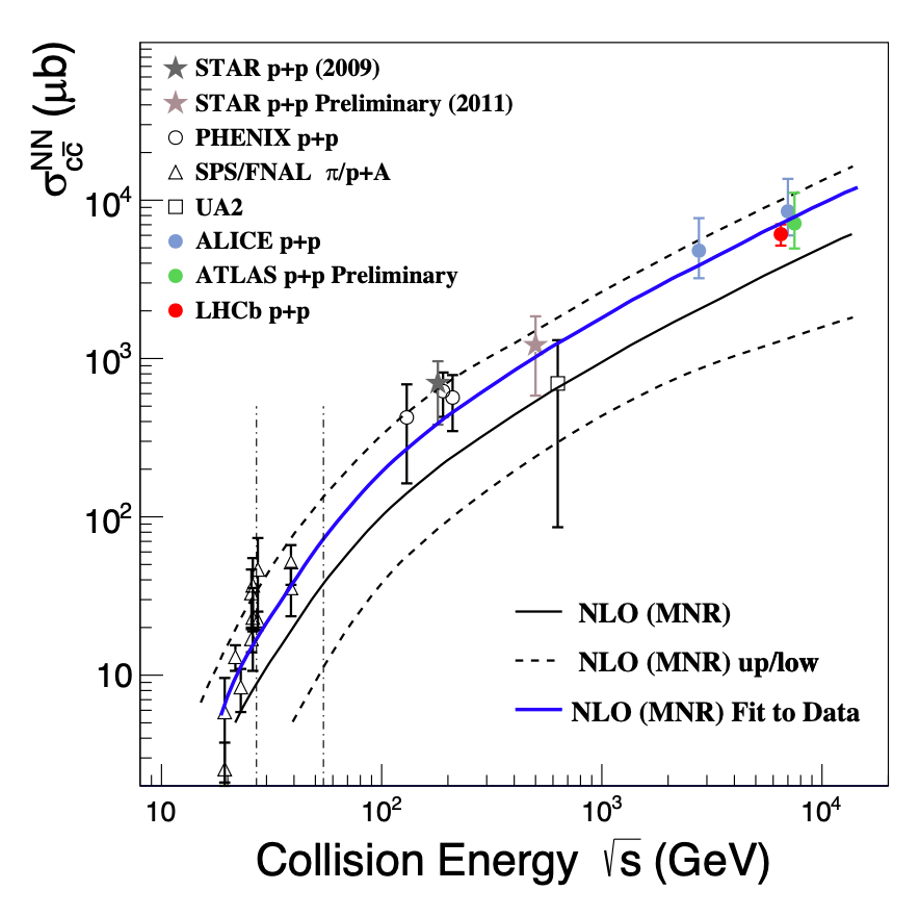
\includegraphics[width=0.8\textwidth,clip]{figures/Chapter4/CharmXsession.png}
    \end{center}
    \caption[c夸克截面拟合结果]{c夸克截面拟合结果,拟合曲线为NLO(MNR)理论计算曲线}
    \label{fig:Charm_Xsection}
\end{figure}
\begin{table}[h!]
    \centering
    \caption{\sNN = 54.4 GeV 金-金对撞中不同中心度下$N_{bin}$的值}
    \label{tab:Nbin}
    \begin{tabularx}{0.8\textwidth} {
    | >{\centering\arraybackslash}X  |>{\centering\arraybackslash}X | }
    \hline
    Centrality & $N_{bin}$ \\
    \hline
    0-80\% & 257.20 \\
    \hline
    0-10\% & 811.80 \\
    \hline
    10-40\% & 342.06 \\
    \hline
    40-80\% & 51.22 \\
    \hline
    \end{tabularx}
\end{table}

测量的初期在如何对c夸克的贡献进行归一化的时候遇到了问题,最开始产生的源自c夸克的双电子模拟谱和STAR BES-1的结果进行比较时发现两边的结果无法匹配,\sNN = 54.4 GeV的结果甚至低于\sNN = 39的c夸克的双轻子模拟谱的结果。后来经过和STAR之前\sNN = 200 GeV 金-金以及质子-质子对撞中的结果进行比较,发现在BES-1的分析和的\sNN = 200 GeV 金-金以及质子-质子对撞的分析当中在对源自c夸克的双电子模拟谱进行模拟的时候采用了两种不同的方法来决定$N_{evt}$的数目。这两种方法分别是:
\begin{itemize}
    \item[inclusive charm method] : $N_{evt}$为在进行模拟时至少有一个c或者 ${\rm \bar{c}}$夸克的事例数
    \item[2 c string method] : $N_{evt}$为在模拟时同时有一个c string 和 ${\rm \bar{c}}$ string的事例数 
\end{itemize}
inclusive charm method 被应用在了\sNN = 200 GeV 金-金以及质子-质子对撞的分析当中,而 2 c string method 被应用在了BES-1的分析当中。

对于双轻子测量来说,之所以要做$1/N_{mb}$的归一化是因为测量的是在一个最小无偏对撞中的双轻子的产额,所以在做模拟的归一化时,所用的总事例数$N_{evt}$应该满足式\ref{eq:N_decay}。这样选取$N_{evt}$就应该和我们计算$\sigma_{c\bar{c}}$时的方法相同。在测量$\sigma_{c\bar{c}}$时是通过测量open charm的产额确定其在中间快度区域的截面后再去反推在全空间的截面。所以$N_{evt}$应该是在模拟当中可以发现open charm的事例数。而在进一步的检查当中发现在PYTHIA6的模拟当中如果事例里面没有2 charm string仍然可以在末态的粒子当中找到来源于open charm的电子对。所以\sNN = 200 GeV测量中使用的确定$N_{evt}$更加合理。为了对这种方法进行验证,在用这种方法模拟产生\sNN = 200 GeV质子-质子对撞当中的重味夸克半轻子衰变的双轻子谱后和STAR之前发表的\sNN = 200 GeV质子-质子对撞中的双轻子谱进行比较,发现可以很好的描述之前的测量数据。所以inclusive charm method被确定为最后的$N_{evt}$数目的选择方法。
\begin{equation}
    \label{eq:N_decay}
    N_{mb} = N_{evt}*\frac{\sigma_{mb}}{\sigma_{c\bar{c}}}
\end{equation}
